% Double-blind review copy for ICST 2027 (Research Papers track, deadline 2 Nov 2026).
% Shares every section file with main.tex; the only differences are the anonymous
% author block, the anonymized self-citations and the anonymized artifact mirror.
% Edit content in the shared section files, never here.
\documentclass[10pt,conference,letterpaper]{IEEEtran}

\usepackage{graphicx}
\usepackage{amsmath}
\usepackage{hyperref}
\usepackage{booktabs}
\usepackage{tabularx}
\usepackage{multirow}
\usepackage{tikz}
\usetikzlibrary{arrows.meta,positioning,fit}

% Anonymized self-citations -- citing mansy2026agentic/mansy2026beyond here
% deanonymizes the submission.
\newcommand{\grammarcite}{\cite{anon2026grammar}}
\newcommand{\dartcite}{\cite{anon2026dart}}

% Anonymized artifact mirror (anonymous.4open.science, mirrors the review-mirror branch).
% TODO before submission: replace with the real mirror URL once it exists.
\newcommand{\artifacturl}{https://anonymous.4open.science/r/knowledge-sources-fuzzing-XXXX/}

\title{Where Does an LLM Fuzzer's Domain Knowledge Come From?\\
Human, Code-Read, and Self-Acquired Knowledge for Differential Testing of Typed Deserializers}

\author{
\IEEEauthorblockN{Anonymous Author(s)}
\IEEEauthorblockA{Submission under double-blind review}
}

\hypersetup{pdfauthor={},pdftitle={Where Does an LLM Fuzzer's Domain Knowledge Come From?}}

\begin{document}

\maketitle

\begin{abstract}
An LLM-guided refinement loop for differential testing of Dart JSON
deserializers found divergence in 2.9\% of generated documents on its own,
but in 28.8\% when a human gave it four observations from a manual
characterization: the bottleneck was domain knowledge, and it came from a
person. We ask whether the fuzzer can acquire that knowledge itself. Holding
the loop fixed and varying only a 1{,}500-character knowledge slot, we
compare sources in a pre-registered study: none, the human's observations,
a summary written by an LLM agent that reads the deserializers' code, and a
summary written by an agent that designs and runs 20 black-box probe
documents. On Dart ($n{=}5$ seeds per arm), human knowledge reaches 30.9\%,
code-read knowledge 11.6\% and no knowledge 1.5\% (each pair
$p \approx 0.008$, Holm-adjusted $p \approx 0.048$). Unguided probing
reaches 10.5\%, not detectably above no knowledge ($p \approx 0.69$): its
probes never remove a required top-level field or leave the
64-bit integer range, and it
succeeds on one seed in five, by accident. A pre-registered extension tests
two remedies. Requiring the agent to cover generic test categories first
raises probing to 20.2\% ($p \approx 0.032$ against no knowledge;
$0.16$ after correction across six tests), with the missing-field pattern
found in every run; a larger model raises it to 12.1\%. Neither reaches
the human arm's mean, and both still leave the integer-overflow pattern mostly
unfound, because the probes never reach it. Across all arms, which known
divergence patterns the loop finds tracks which facts the knowledge states.
On Kotlin (Gson, Moshi, kotlinx.serialization, Jackson), where divergence is
common, probing helps without guidance (67.1\% against 50.0\% over ten
seeds, $p \approx 0.007$) and more with it (81.6\%). Self-characterization
works where interesting behaviour is dense, and needs systematic coverage
where it is narrow.

\end{abstract}

\begin{IEEEkeywords}
fuzzing, differential testing, large language models, domain knowledge, black-box testing, JSON deserialization, Dart, Kotlin
\end{IEEEkeywords}

\section{Introduction}

LLM-guided fuzzers are often described as bringing their own knowledge: a
model trained on large amounts of code is expected to know what inputs
stress a parser or a compiler~\cite{deng2023titanfuzz,xia2024fuzz4all}. A
previous study of differential testing for Dart JSON
deserialization~\dartcite{} found the opposite in a controlled setting. A
bounded refinement loop, in which an LLM writes and rewrites a
Hypothesis~\cite{maciver2019hypothesis} generator from a score-only
feedback signal, found cross-implementation divergence in only 2.9\% of
generated documents, against 22.2\% for a hand-built static generator.
Richer feedback, incremental mutation and a larger model did not close the
gap. Four observations taken from a thirteen-case manual characterization
did: with them in the prompt, the same loop reached 28.8\%. But it never
found a divergence it had not been told about. The bottleneck was domain
knowledge, and it came from the researchers.

This paper asks where else that knowledge can come from. A human
characterization is slow and requires an expert; if a fuzzer is to be
applied to a new ecosystem, the knowledge has to be obtained some other way.
Two automated sources are natural. An agent can \emph{read the code} of the
implementations under test and summarize what it finds, as white-box LLM
testing tools do~\cite{yang2024whitefox,yang2025kernelgpt,vadayath2026aijon}.
Or an agent can \emph{run experiments}: design a small number of probe
documents, observe how each implementation handles them, and write down what
it learned. The second is what the researchers did by hand in that study, and it
needs no source code, which matters when the implementations are closed,
generated at compile time, or reflective. We call it \emph{black-box
self-characterization}.

We compare these sources under control. The refinement loop, model,
sampling settings and feedback are those of that study, unchanged;
the only thing that differs between arms is the text in a single knowledge
slot of the prompt, capped at 1{,}500 characters. The four arms are
\emph{none}, \emph{human} (the four observations, verbatim),
\emph{code} (a summary written after reading the four paths'
deserialization code) and \emph{probe} (a summary written after running 20
probe documents in two rounds). The design, seeds, tests and decision rules
were fixed and committed before any code or API spend, and every later
change is recorded in a deviations log with its reason. We ask:

\begin{itemize}
\item \textbf{RQ1 (acquisition).} Can a probing agent acquire knowledge
that closes the refinement gap as well as human knowledge does? We answer
this on Dart, where the answer key is known.
\item \textbf{RQ2 (sources).} How do the four knowledge sources compare in
divergence rate, in which known divergence patterns they lead to, and in
cost?
\item \textbf{RQ3 (transfer and discovery).} On an ecosystem with no human
characterization, Kotlin with four widely used JSON libraries, does probing
knowledge help, does it rediscover a known behavior, and does it find
anything new?
\item \textbf{RQ4 (remedies, pre-registered extension).} If unguided
probing fails, is it because the probes miss the relevant inputs or because
the model is too weak? We test a probing agent told to cover generic test
categories first, and the unchanged agent with a larger model.
\end{itemize}

Our findings are:

\begin{itemize}
\item On Dart, knowledge sources are clearly ordered: human (30.9\%) above
code-read (11.6\%) above none (1.5\%), each difference significant after
correction. Probing reaches 10.5\% on average but is not distinguishable
from no knowledge ($p \approx 0.69$). It is all-or-nothing: 49\% on the one
seed whose probes hit a divergence, at most 1.3\% on the others.
\item The divergence patterns each arm finds follow the facts its summary
states. Every code summary states that two paths accept a non-integer
\texttt{id}, and every code run finds the \texttt{id} pattern; no code
summary states that one path substitutes an empty list for a missing
\texttt{tags} field, and one code run in five finds that pattern. No probe summary mentions non-integer \texttt{id}
values, and no probe run finds the \texttt{id} pattern.
\item On Kotlin, where 11--14 of 20 probes diverge on every seed, probing
knowledge helps: 67.1\% against 50.0\% over ten seeds ($p \approx 0.007$),
using a replication declared before it ran.
\item Both remedies help on Dart. Systematic probing reaches 20.2\%
($p \approx 0.032$ against none; $0.16$ after Holm correction across the
six declared tests), and every one of its runs finds the missing-field
pattern; a larger model reaches 12.1\%. Neither reaches the human arm's mean.
The agents covered the first checklist items thoroughly and never reached
the 64-bit boundary items, so the integer-overflow pattern stayed mostly
unfound: coverage decides what is learned, and a budget of 20 probes does not
cover enough.
\item Triage of every Kotlin divergence class found documented defaults and
known issues, including the Gson null-safety bypass that served as our
answer key, and one standards violation in kotlinx.serialization's strict
mode, which we reported upstream.
\end{itemize}

The overall lesson is conditional. Black-box self-characterization works
when the behaviors worth knowing are easy to stumble on. When they are
narrow, which is where an unguided fuzzer also fails and knowledge matters
most, it works only as far as its probes are made to reach them. The data,
agents, prompts and analysis are available at \url{\artifacturl}.

\section{Related Work}

\textbf{LLM-driven fuzzing and test generation.} LLMs have been used as
zero-shot input generators for deep-learning libraries~\cite{deng2023titanfuzz},
as universal fuzzers across languages~\cite{xia2024fuzz4all}, and to escape
coverage plateaus in search-based test generation~\cite{lemieux2023codamosa}.
These systems draw on what the model already knows from pre-training. Our
earlier studies put such a model inside a bounded, coverage-free refinement
loop, first against C parsers~\grammarcite{} and then against Dart
deserializers with a differential oracle~\dartcite{}; the second is where
the knowledge gap studied here was measured.

\textbf{Knowledge from reading code.} WhiteFox~\cite{yang2024whitefox} has
an LLM agent read compiler optimization source code and write requirements
for test programs that trigger it. KernelGPT~\cite{yang2025kernelgpt}
infers syscall specifications from kernel source for Syzkaller.
DiffSpec~\cite{rao2024diffspec} generates differential tests from natural-language
specifications and code artifacts. AIJon~\cite{vadayath2026aijon} generates
IJON annotations from source and finds them roughly on par with human-written
ones in a coverage-guided fuzzer. All of these derive knowledge by reading
code or specifications, for coverage or for test requirements. None compares
knowledge sources under control, and none acquires knowledge by running the
target. Our \emph{code} arm is a small, controlled instance of this family;
our \emph{probe} arm is the black-box alternative.

\textbf{Differential testing of JSON processing.} Differential
testing~\cite{mckeeman1998differential} of JSON parsers across languages has
found many semantic discrepancies at the parsing level, text to
tree~\cite{moller2024crosslanguage}. JsonATG~\cite{wang2025jsonatg} uses a
multi-agent LLM pipeline to generate bug-triggering tests for Java JSON
libraries. We test \emph{typed binding}, tree to class, where divergences
come from how each library maps JSON onto a language's types and
null-safety rules, and we compare four libraries on one class in two
ecosystems.

\textbf{Known Kotlin behaviour.} That Gson bypasses Kotlin null-safety is a
long-standing known issue~\cite{gsonissue1657}, which we use as an answer
key: a behaviour the agents should rediscover without being told.

\section{Method}

Figure~\ref{fig:overview} shows the setup. Four knowledge sources feed one
slot in the prompt of an otherwise fixed refinement loop; the loop's
generators are scored by a differential harness over four deserialization
paths.

\begin{figure}[t]
\centering
\resizebox{\columnwidth}{!}{%
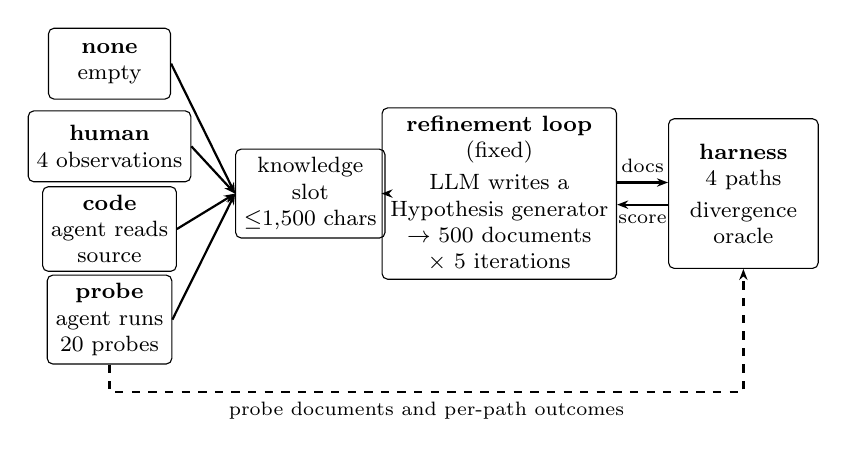
\begin{tikzpicture}[
  font=\footnotesize,
  box/.style={draw, rounded corners=2pt, align=center, inner sep=3pt},
  src/.style={box, minimum width=1.55cm, minimum height=0.9cm},
  arr/.style={-{Stealth[length=4pt]}, thick}]
\node[src] (none)  at (0,3.0)  {\textbf{none}\\empty};
\node[src] (human) at (0,1.95) {\textbf{human}\\4 observations};
\node[src] (code)  at (0,0.9)  {\textbf{code}\\agent reads\\source};
\node[src] (probe) at (0,-0.25) {\textbf{probe}\\agent runs\\20 probes};
\node[box, minimum width=1.5cm, minimum height=1.1cm] (slot) at (2.55,1.35) {knowledge\\slot\\$\le$1{,}500 chars};
\node[box, minimum width=2.1cm, minimum height=1.9cm] (loop) at (4.95,1.35)
  {\textbf{refinement loop}\\(fixed)\\[2pt]LLM writes a\\Hypothesis generator\\$\to$ 500 documents\\$\times$ 5 iterations};
\node[box, minimum width=1.9cm, minimum height=1.9cm] (harness) at (8.05,1.35)
  {\textbf{harness}\\4 paths\\[2pt]divergence\\oracle};
\foreach \n in {none,human,code,probe} \draw[arr] (\n.east) -- (slot.west);
\draw[arr] (slot) -- (loop);
\draw[arr] ([yshift=4pt]loop.east) -- node[above, font=\scriptsize]{docs} ([yshift=4pt]harness.west);
\draw[arr] ([yshift=-4pt]harness.west) -- node[below, font=\scriptsize]{score} ([yshift=-4pt]loop.east);
\draw[arr, dashed] (probe.south) |- ++(0,-0.35) -| node[pos=0.25, below, font=\scriptsize]{probe documents and per-path outcomes} (harness.south);
\end{tikzpicture}}
\caption{Study design. Only the knowledge slot differs between arms. The
probing agent runs its probes through the same harness the loop is scored
by.}
\label{fig:overview}
\end{figure}

\subsection{Targets and oracle}

Both targets decode the same logical record: a non-null integer
\texttt{id}, a string \texttt{amount}, a nullable string \texttt{name}, a
\texttt{status} enum with three values, a non-null list of strings
\texttt{tags}, and a nullable recursive \texttt{child}. Each generated
document is run through four deserialization paths in one
long-lived harness process. A document \emph{diverges} if one path accepts
it and another rejects it, or if all accept but decode different values.
Values are compared through a canonical JSON rendering of the decoded
object built only from primitives, so that the comparison itself cannot
fail. The harness speaks newline-delimited JSON on standard input and output,
with each document base64-encoded, so arbitrary bytes reach the paths
unchanged. The primary metric, as in the previous study, is the percentage
of all generated documents that diverge.

\textbf{Dart} reuses the previous study's harness unchanged~\dartcite: hand-written
parsing, \texttt{json\_serializable}~\cite{jsonserializable2026},
\texttt{freezed}~\cite{freezed2026} and
\texttt{built\_value}~\cite{builtvalue2026}, on Dart
3.13.2~\cite{dart2026lang}. All four receive the output of one shared
\texttt{jsonDecode}, so invalid JSON is rejected identically before any
path runs. Two divergence patterns are known (written in path order):
\texttt{RAAR}, where the two paths that decode \texttt{id} through
\texttt{num.toInt()} accept a large integer literal that
\texttt{jsonDecode} has turned into a double, and saturate it; and
\texttt{RRRA}, where \texttt{built\_value} alone accepts a document with
\texttt{tags} missing and substitutes an empty list.

\textbf{Kotlin} uses a new harness with the same protocol and four libraries
at their documented defaults: Gson~\cite{gson2026},
Moshi with its generated adapter~\cite{moshi2026},
kotlinx.serialization~\cite{kotlinxserialization2026} and Jackson with its
Kotlin module~\cite{jacksonkotlin2026}. The record is an idiomatic data
class with no default values and no configuration beyond the annotations each
library needs to run. Unlike Dart, each library parses the raw text itself,
so all four run on every input and syntax-level divergence counts. The known
answer key is the Gson null-safety bypass~\cite{gsonissue1657}: Gson
constructs objects without Kotlin's constructor checks, so a missing or
\texttt{null} value for a non-null property is accepted as \texttt{null}.
Divergence that follows from a documented default is labeled as such and
never called a bug.

\subsection{The refinement loop}

The loop is the previous study's score-only loop~\dartcite, unchanged
except for one setting. Each of five iterations asks \texttt{gpt-4.1-mini}~\cite{openai2025gpt41}
(temperature 0.2) for a Hypothesis generator of JSON documents, draws 500
documents from it in a restricted sandbox, and reports back how many
diverged. The prompt describes the schema and the four paths, gives the
score and a generic strategy hint (vary one thing at a time: a wrong type, a
missing field, a boundary value), and asks for a new generator. A test
rebuilds all 100 prompts committed by the previous study's score-only and
knowledge arms byte for byte. The one change is the output-token limit,
raised from 2{,}500 to 8{,}000 for every arm before any experiment data, after
a pilot lost four of five generators to truncation; no response in the main
study was truncated, and one of the extension's 75 was.

\subsection{Knowledge arms}

Each arm fills one knowledge slot in the prompt: a one-sentence header naming
the source, followed by a body of at most 1{,}500 characters.

\textbf{None.} The slot is empty.

\textbf{Human} (Dart only). The four observations from the previous study,
verbatim (1{,}291 characters): that invalid JSON never reaches the paths;
that \texttt{built\_value} alone accepts a missing \texttt{tags} and uses
an empty list; that wrong types and nulls are rejected by all four in every
case tried; and that two paths decode \texttt{id} as \texttt{num.toInt()},
which saturates for integer literals outside the 64-bit range. The label
means that the researchers produced this knowledge outside the pipeline,
from documents they chose, rather than an agent inside it.

\textbf{Code} (Dart only). An agent reads a fixed, per-seed identical set
of nine source files, about 17{,}000 characters: each path's model and its
generated \texttt{*.g.dart} code. It then writes a numbered list of
behavioral observations. For Kotlin no comparable source exists: Gson and
Jackson are reflective and kotlinx.serialization generates bytecode with a
compiler plugin. That asymmetry is itself a practical argument for black-box
probing.

\textbf{Probe.} An agent designs up to 20 probe documents in two rounds, at
most 12 then the rest, written as raw text so that non-JSON probes are
possible. Each probe runs through the real harness, and the agent sees, per
path, whether it accepted or rejected the document, the exception type, and
the decoded value. After the second round it writes a numbered list of
observations.

Both agents use the same model and settings as the loop and see the same
target description and strategy hint as the \emph{none} arm, so each starts
from exactly the \emph{none} arm's a priori information. If a summary is
over the cap, one shortening call follows, then a cut at the last line break
under the cap; the cut applied in 19 of 20 acquisitions (mean body 1{,}422
characters). Knowledge is acquired once per seed, so its quality varies
across seeds, and that variance is part of the result.

\subsection{Extension: two remedies for probing}
\label{sec:extension}

After the main results, we declared an extension in the deviations log and
published it before any of its runs, with two new arms and no new seeds for
any existing arm.

\textbf{Systematic probing} (\emph{sysprobe}; Dart and Kotlin). The probing
agent, model, budget and cap are unchanged. Its prompt adds the checklist in
Fig.~\ref{fig:checklist}, and its summary must end with a line listing the
categories no probe covered. Every item is a standard, schema-independent
category from category-partition testing~\cite{ostrand1988category} and
boundary-value analysis~\cite{myers2011art}, and
none names a field, path or library; we disclose that it was written by an
author who knew the answer key. The knowledge header is the same as for
\emph{probe}, so only the body differs.

\textbf{A larger prober} (\emph{probe-gpt41}; Dart). The unchanged probing
agent and prompts, with \texttt{gpt-4.1} for knowledge acquisition only; the
loop stays \texttt{gpt-4.1-mini}.

Both arms use the seeds of the corresponding \emph{probe} arm. The declared
tests are systematic probing against none on Dart (primary), against unguided
probing, human and code on Dart, and against none and unguided probing on
Kotlin, with a Holm correction across these six; and the larger prober
against unguided probing and against none, with a Holm correction across
the two.

\begin{figure}[t]
\centering
\fbox{\begin{minipage}{0.94\columnwidth}
\footnotesize
Probe systematically. Spend your probes on these categories first; they apply
to any JSON schema, and each probe should change one thing in an otherwise
valid document:
(1) a required field missing;
(2) a non-nullable field set to null;
(3) a field with a value of the wrong JSON type;
(4) a numeric field at a representation boundary: a fraction, an exponent
form, and integers just beyond the 32-, 53- and 64-bit ranges;
(5) an enum-like field with an unknown value, and with a case variant;
(6) an extra unknown key, and a duplicate key;
(7) the same kinds of change inside a nested object;
(8) text that is not strict JSON: single quotes, an unquoted value, a
trailing comma, NaN, and a raw control character inside a string.
Prefer breadth across categories over repetition.
\end{minipage}}
\caption{The checklist added to the systematic probing agent's prompt
(abridged; the full text is in the artifact).}
\label{fig:checklist}
\end{figure}

\subsection{Design and analysis}

The study was pre-registered in a design document committed before any code
or API spend; later changes are listed in a dated deviations log. Dart arms
run on seeds 700--704 and Kotlin arms on 800--804. Pilots used seeds outside
these ranges, and the probing and code agents' prompts were frozen after one
pilot change: both agents were given the refinement prompt's existing
strategy hint, which the \emph{none} arm already sees.

For each run, iterations whose generator failed validation contribute no
documents, as in the previous study. We compare arms with an exact two-sided
Mann--Whitney U test and report the mean difference and Cliff's $\delta$.
The primary test is \emph{probe} against \emph{none} on Dart, with
\emph{probe} against \emph{human} co-primary; all six Dart pairs are reported
with a Holm correction alongside raw $p$-values. The Kotlin primary is
\emph{probe} against \emph{none}. A $p \geq 0.05$ is reported as ``not
detected at $n{=}5$'', not as ``no effect''. A claim of comparability to
human knowledge requires $|\delta| < 0.33$ in addition to $p \geq 0.05$.
Replication on fresh seeds was allowed only if declared in the log before
it ran. Secondary measures are pattern recall (the fraction of runs that
find each known pattern at least once) and cost in calls and tokens.

\section{Results}

\subsection{RQ1 and RQ2: knowledge sources on Dart}

Table~\ref{tab:dart} gives the divergence rate of every run.
Human knowledge reproduces our previous result on fresh seeds (30.9\%,
against 28.8\% before). Code-read knowledge sits between human and none, and
every run in each of these three arms is ordered: all five human runs exceed
all five code runs, which exceed all five \emph{none} runs.

\begin{table}[t]
\centering
\caption{Dart divergence rate per run (\% of all generated documents),
seeds 700--704 in order.}
\label{tab:dart}
\begin{tabular}{lrl}
\toprule
Arm & Mean & Per seed \\
\midrule
none  & 1.45  & 3.40, 0.00, 0.67, 3.20, 0.00 \\
human & 30.89 & 21.60, 29.65, 48.30, 29.13, 25.75 \\
code  & 11.55 & 10.10, 16.04, 8.40, 13.40, 9.80 \\
probe & 10.51 & 1.07, \textbf{49.27}, 1.27, 0.93, 0.00 \\
\bottomrule
\end{tabular}
\end{table}

\begin{table}[t]
\centering
\caption{Pairwise Dart comparisons: difference in mean rate (percentage
points), exact two-sided Mann--Whitney U, Holm-adjusted $p$, Cliff's
$\delta$. $n{=}5$ per arm.}
\label{tab:dart-tests}
\begin{tabular}{lrrrr}
\toprule
Comparison & $\Delta$ & $p$ & $p_{\mathrm{Holm}}$ & $\delta$ \\
\midrule
probe$-$none (primary) & $+9.05$  & 0.690 & 0.690 & $+0.20$ \\
probe$-$human (co-prim.) & $-20.38$ & 0.151 & 0.452 & $-0.60$ \\
human$-$none & $+29.43$ & 0.008 & 0.048 & $+1.00$ \\
code$-$none & $+10.09$ & 0.008 & 0.048 & $+1.00$ \\
code$-$human & $-19.34$ & 0.008 & 0.048 & $-1.00$ \\
probe$-$code & $-1.04$  & 0.151 & 0.452 & $-0.60$ \\
\bottomrule
\end{tabular}
\end{table}

\textbf{RQ1.} Probe knowledge is not detectably better than none
(Table~\ref{tab:dart-tests}, $p \approx 0.69$, $\delta = +0.20$). By the
pre-registered rule this is ``not detected at $n{=}5$'', and the claim of
comparability to human knowledge is not supported ($\delta = -0.60$).
The mean hides the shape of the distribution. Four probe runs stay at or
below 1.3\%, in the range of \emph{none}; one, seed 701, reaches 49.3\%,
above every human run. Seed 701 is the only seed whose probing phase
observed a divergence at all: one of its 100 probes across five seeds
diverged (\texttt{built\_value} accepting a nested \texttt{tags: null}), and
its summary reported it. The probes of the other four seeds diverged on
none of their 20 documents. When probing sees nothing, its summary is a
confident description of agreement, and the loop behaves as if it had no
knowledge. Summaries can also overgeneralize: one states that no
implementation throws an undocumented exception, although three of the four
paths throw Dart's private \texttt{\_TypeError} on the probes it ran.

\textbf{RQ2.} Human $>$ code $>$ none holds with the largest possible
effect in every pair and survives the Holm correction. Code-read knowledge is
the stable middle: it varies between 8.4\% and 16.0\% and never fails.
Probe knowledge has a similar mean but the opposite profile. The two are not
distinguishable at $n{=}5$.

\begin{table}[t]
\centering
\caption{Dart pattern recall. \emph{Stated}: summaries (of five) that state
the fact behind the pattern. \emph{Found}: runs (of five) that found the
pattern at least once.}
\label{tab:recall}
\begin{tabular}{lcccc}
\toprule
& \multicolumn{2}{c}{\texttt{RAAR} (\texttt{id})} & \multicolumn{2}{c}{\texttt{RRRA} (\texttt{tags})} \\
Arm & stated & found & stated & found \\
\midrule
none  & --   & 3/5 & --   & 3/5 \\
human & 5/5  & 5/5 & 5/5  & 5/5 \\
code  & 5/5  & 5/5 & 0/5  & 1/5 \\
probe & 0/5  & 0/5 & 1/5$^{*}$ & 4/5 \\
\bottomrule
\end{tabular}\\[2pt]
{\footnotesize $^{*}$Seed 701 states that \texttt{built\_value} accepts
\texttt{tags: null}: related, but not the missing-field fact.}
\end{table}

\textbf{What the knowledge contains decides what is found.}
Table~\ref{tab:recall} compares, for each Dart pattern, whether an arm's
knowledge states the fact behind it with how many runs found it. Every
code summary states that two paths accept a non-integer \texttt{id} through
\texttt{num.toInt()}; every code run finds \texttt{RAAR}. None of them
mentions large integers or overflow, which is the other half of the
mechanism, but a generator that varies \texttt{id} types reaches it anyway.
No code summary states that \texttt{built\_value} substitutes an empty
list for a missing \texttt{tags}, and one code run finds \texttt{RRRA}.
The probe summaries are the mirror image: none mentions a non-integer
\texttt{id}, and no probe run finds \texttt{RAAR}, not even the one at
49\%, whose divergences are all \texttt{RRRA}. No arm found a Dart pattern
outside the answer key. The loop exploits what it is told; it does not
extend it, which is what our previous study observed for human knowledge.

\textbf{Cost.} A \emph{none} or \emph{human} run takes five calls, about
\$0.014 at list prices. Code knowledge adds two calls per seed (\$0.004) and
probing four (\$0.006), plus 20 harness executions. Knowledge acquisition is
cheap compared with the loop; the whole study, including pilots, cost less
than one US dollar.

\subsection{RQ3: Kotlin}

On Kotlin the picture is reversed. The probing agents observed divergence
on 11 to 14 of their 20 probes on every seed: the four libraries disagree
about wrong types, nulls, unknown keys, unknown enum constants and lenient
syntax. The summaries record these disagreements, and the loop uses them
(Table~\ref{tab:kotlin}).

\begin{table}[t]
\centering
\caption{Kotlin divergence rate (\% of all documents), probe vs.\ none.
The replication on seeds 805--809 was declared before it ran.}
\label{tab:kotlin}
\begin{tabular}{lrrrr}
\toprule
Seeds & none & probe & $p$ & $\delta$ \\
\midrule
800--804 (pre-registered) & 45.77 & 64.34 & 0.095 & $+0.68$ \\
805--809 (replication)    & 54.14 & 69.92 & 0.056 & $+0.76$ \\
pooled, $n{=}10$ per arm  & 49.95 & 67.13 & \textbf{0.007} & $+0.70$ \\
\midrule
pooled, RFC 8259-valid only & 42.55 & 56.49 & 0.075 & $+0.48$ \\
\bottomrule
\end{tabular}
\end{table}

The pre-registered comparison on seeds 800--804 had a large effect but did
not reach significance ($p \approx 0.095$). As the design allowed, we
declared a replication on fresh seeds before running it; it showed the same
direction and size ($+15.8$ points, $\delta = +0.76$), and the pooled
comparison over ten seeds per arm is significant ($p \approx 0.007$). We
report all three rows: neither half is significant alone.

The last row restricts both arms to documents that are valid JSON under
RFC~8259~\cite{rfc8259}. The harness's own validity label turned out to be
too lenient during triage (Section~\ref{sec:triage}), so this row uses a
strict parser applied after the fact, as recorded in the deviations log.
The effect shrinks ($\delta = +0.48$, $p \approx 0.075$): part of the
probe arm's advantage comes from malformed input that some libraries accept
and others do not.

Every Kotlin run in both arms, including all ten without knowledge,
rediscovered the Gson null-safety bypass, in 114 to 970 documents per run.
On Kotlin this answer key is too easy to separate the arms.

\subsection{Triage of Kotlin divergences}
\label{sec:triage}

We grouped every divergent Kotlin document by pattern and exception types,
reproduced each group by hand with a minimal document that changes one
field of a valid record, and checked the result against each library's
documentation and issue tracker. No run produced a value divergence:
whenever all four libraries accepted a document, they decoded the same
value.

Eleven behaviours are documented defaults or known limitations. They are
Gson's null-safety bypass and its mapping of unknown enum constants to
\texttt{null}; Gson and Jackson decoding a missing or \texttt{null}
\texttt{id} as 0, which Jackson's Kotlin module documents as a caveat;
Gson, Moshi and Jackson accepting \texttt{null} elements in a
\texttt{List<String>} (strict null checks are opt-in for Jackson); the coercion
of numbers and booleans to strings; kotlinx.serialization and Jackson rejecting
unknown keys; kotlinx.serialization requiring a nullable property with no
default; Jackson truncating \texttt{1.9} to \texttt{1}; and Gson's lenient
syntax; and two coercions of string values to \texttt{Long}: Jackson reading
an empty string as 0, and Gson and Moshi accepting a numeric string with a
fraction, such as the string \texttt{1.0}.

One behaviour is a standards violation. kotlinx.serialization's
\emph{default}, non-lenient \texttt{Json} accepts raw control characters
(U+0000--U+001F) inside strings, which RFC~8259 forbids and which Jackson
and Dart's \texttt{jsonDecode} reject. We reproduced it outside the harness
on version 1.11.0 and on the latest release candidate, 1.12.0-RC. It had
been reported only inside a generic benchmark issue that was closed as not
planned without comment~\cite{kotlinxissue3273}, and we have prepared a
focused report. The same leniency is why the harness's validity label,
which used kotlinx.serialization's parser, was not RFC-strict.

Two more defects surfaced only in our manual reproductions, not in any run
or probe: Gson saturating an integer literal just above $2^{63}$ to
\texttt{Long.MAX\_VALUE}~\cite{gsonissue1727}, and kotlinx.serialization
wrapping integers modulo $2^{64}$, so that \texttt{18446744073709551617}
decodes as \texttt{1}~\cite{kotlinxissue3267}. Both are known and open. We
do not credit them to the method: like \texttt{RAAR} for the probe arm,
they sit in a narrow numeric region that neither the probes nor the
generators visited.

\section{Discussion}

\textbf{Probing is a search problem with a small budget.} A probing agent
learns only what its probes reveal. On Dart, where divergence requires a
specific field to be absent or an integer literal to leave the 64-bit range,
20 probes chosen by the model's prior found a divergence on one seed in five.
Table~\ref{tab:coverage} classifies all 300 probes by what they change
relative to a valid record. The agents probed the same way on both targets:
mostly valid documents, then one wrong type, an unknown enum constant or an
extra key. On neither target did any probe remove a required top-level field,
use an \texttt{id} near a 53- or 64-bit boundary, or send text that is not
JSON, although probes were raw text precisely to allow that. Wrong types,
unknown enum constants and extra keys never diverged on Dart; on Kotlin they
are exactly where the libraries disagree. The difference between the targets is the density of
divergence near the inputs the model finds natural, not the agent's
behaviour.

\begin{table}[t]
\centering
\caption{What the probes changed, relative to a valid record (a probe can
be in several rows). Seeds: on how many seeds at least one probe did it.}
\label{tab:coverage}
\footnotesize
\begin{tabular}{@{}lrrrr@{}}
\toprule
& \multicolumn{2}{c}{Dart (100 probes)} & \multicolumn{2}{c}{Kotlin (200)} \\
Change & probes & seeds & probes & seeds \\
\midrule
nothing at top level     & 68 & 5/5 & 117 & 10/10 \\
wrong type               & 19 & 5/5 & 48 & 10/10 \\
unknown enum constant    & 6  & 5/5 & 11 & 10/10 \\
extra key                & 6  & 5/5 & 14 & 9/10 \\
null for non-null field  & 1  & 1/5 & 10 & 8/10 \\
nested \texttt{child} changed & 19 & 5/5 & 42 & 10/10 \\
missing required field   & 0  & 0/5 & 0  & 0/10 \\
\texttt{id} near 53/64-bit boundary & 0 & 0/5 & 0 & 0/10 \\
not JSON                 & 0  & 0/5 & 0  & 0/10 \\
\bottomrule
\end{tabular}
\end{table}
The agent's ability to characterize a target is therefore bounded by the
same thing that bounds the fuzzer: the density of interesting behaviour near
the inputs the model finds natural. This is the conditional result in our
title question. Self-acquired knowledge helps when an unguided search would
have found some divergence anyway, and gives nothing where knowledge is most
needed.

\textbf{Negative evidence is misleading.} A probe summary that observed no
divergence does not say ``I did not look at missing fields''; it says that
the implementations behave identically, sometimes with an overgeneralization
that is false. The loop then receives confident but empty knowledge. A
practical probing agent should report what it did \emph{not} test, or be
required to cover categories of perturbation, such as each field missing,
each field null and each numeric boundary, before summarizing. Such a checklist
is itself domain knowledge, so it moves the question rather than removing
it, but it is generic across schemas and cheap to write once.

\textbf{Code reading is reliable but incomplete.} The code arm never failed,
because the facts are in the code whether or not the agent thinks to test
them. It stated the \texttt{num.toInt()} difference in every summary and
found \texttt{RAAR} in every run. It missed \texttt{built\_value}'s
empty-list default, which lives in generated builder code rather than in
the decoding call, and it never connected \texttt{toInt()} to
\texttt{jsonDecode}'s treatment of large literals, which lives in the SDK and
was not in its reading list. Reading more code would help, at the cost of the
fixed budget. On Kotlin the arm could not be run at all: the equivalent logic
is reflective or compiler-generated.

\textbf{Combining sources.} Code reading and probing fail differently. Code
reading states what the implementation does wherever the logic is visible,
but misses behaviour that lives outside its reading list, such as the SDK's
number parsing. Probing observes behaviour end to end, including such
interactions, but only where it looks. A natural combination, which we did
not evaluate, is to let code reading propose where to probe, and probing
confirm or refute what code reading claims. That would also address the
overgeneralization we observed, because a claim of agreement would then have
to name the probes that support it.

\textbf{For practitioners.} Where a human characterization exists, use it:
it was the best source by a wide margin and costs nothing at run time. Where
source is available, a code-reading summary gives a dependable improvement
for a few cents. A probing agent is worth running first to learn whether
disagreement is common; if its probes find none, treat its summary as
uninformative, not as evidence of agreement.

\subsection{Threats to validity}

\textbf{Sample size.} Each arm has five seeds, the smallest size at which an
exact Mann--Whitney test can reach $p < 0.05$. The primary Dart result is a
non-detection, and the bimodal probe distribution means a larger sample
would most likely estimate how often probing hits, not remove the
variance. The Kotlin result relies on a pre-declared replication and is
weaker on RFC-valid documents alone ($p \approx 0.075$).

\textbf{Knowledge quality is uncontrolled.} Summaries are capped at the
same length but differ in accuracy, which is the variable under study. The
cap was applied by cutting in 19 of 20 acquisitions, which drops the last
observations; a different enforcement rule could change individual
summaries.

\textbf{One model family and one probe budget.} All agents and the loop use
\texttt{gpt-4.1-mini}, and the probe budget of 20 is a choice. A stronger
model or a larger budget might probe more widely; the previous study found
that a larger model alone did not close the gap.

\textbf{Post-data change.} The Kotlin harness's validity label was found to
be lenient after the data existed. It affects only a secondary metric, which
we recompute with a strict parser; the harness is unchanged so that the
committed runs stay reproducible. The output-token limit was raised before
any experiment data, for every arm.

\textbf{Non-determinism and model drift.} The API is not seedable, so a
seed labels a run rather than fixing it; re-running reproduces the procedure,
not the documents. All prompts, responses, generators and per-document
results are committed so that every reported number can be recomputed without
calling the API. A hosted model may also change over time; all runs were
made within two days, and the model identifier is recorded in each
manifest.

\textbf{Answer keys and generality.} Pattern recall is measured against two
known Dart patterns and one known Kotlin behaviour; a source could help in
ways these keys do not capture. Both targets decode one small record schema
from JSON, with four paths each. The conditional result, that probing helps
where divergence is dense, is a hypothesis for other formats and schemas, not
a finding about them.

\textbf{Harness fidelity.} The Dart arms reuse the previous study's harness
binary and loop; a test rebuilds all 100 of its committed prompts byte for
byte, and its committed results summarize identically under the ported
code. The Kotlin harness is new; each behaviour the paper reports was
reproduced with a minimal hand-written document, and the control-character
behaviour also in a standalone program outside the harness, on two library
versions.

\textbf{Construct.} ``Divergence'' counts documents, and on Kotlin many of
them express the same few documented behaviours. Pattern recall and the
triage are reported alongside the rate for this reason.

\section{Conclusion}

An LLM refinement loop for differential testing depends on domain knowledge
it does not have. We compared four sources of that knowledge under control,
changing nothing but a 1{,}500-character slot in the prompt. A human
characterization was best, a summary written from reading the code was a
reliable second, and a summary written from 20 black-box probes was
all-or-nothing on Dart, where divergence is rare, and clearly helpful on
Kotlin, where it is common. Across arms, the divergence patterns found
matched the facts the knowledge stated, and no arm went beyond them.
Self-characterization is therefore not a substitute for knowledge where
knowledge matters most; making it one will need probing that is
systematic about what it covers and honest about what it did not.

\section*{Data Availability}

The design and deviations log, harnesses, agents, prompts, every generated
document and summary, and the analysis scripts are available at
\url{\artifacturl}.


\bibliographystyle{IEEEtran}
\bibliography{references}

\end{document}
